%\documentclass{vldb}
%\documentclass{sig-alternate}
\documentclass{article}
\usepackage{fullpage}

\frenchspacing
\sloppy
\pdfpagewidth=8.5in
\pdfpageheight=11in

\usepackage[english]{babel}
\usepackage{blindtext}
\usepackage[T1]{fontenc}

\usepackage{amsmath}
\usepackage{comment}
\usepackage{amssymb}
\usepackage{amsthm}
\usepackage[hide]{chato-notes}
\usepackage{cite}
\usepackage{color}
\usepackage{graphicx}
\usepackage{xspace}
\usepackage{algorithmic}
\algsetup{linenosize=\small}
\usepackage[ruled,lined,linesnumbered,noend]{algorithm2e}
\newcommand\mycommfont[1]{\scriptsize\rmfamily\itshape\textcolor{black}{#1}}
\SetCommentSty{mycommfont}
\usepackage{epsfig}
\usepackage{epstopdf}
\usepackage[font={bf}]{caption}
%\DeclareCaptionType{copyrightbox}
\usepackage{xcolor}
\usepackage{balance}
\usepackage{enumitem}
\usepackage{framed}

\usepackage{hyperref}
\hypersetup{
	colorlinks,breaklinks,
	urlcolor=[rgb]{0,0.25,0.75},
	linkcolor=[rgb]{0,0.25,0.75},
	citecolor=[rgb]{0,0.25,0.75}
}
\DeclareMathOperator*{\argmin}{arg\,min}
\DeclareMathOperator*{\argmax}{arg\,max}

\newcommand{\laks}[1]{{\color{brown} [\text{Laks: } \sf #1]}}
\newcommand{\weic}[1]{{\color{blue} [\text{Wei Chen: } \sf #1]}}
\newcommand{\weil}[1]{{\color{magenta} \textsf{[Wei Lu: #1]}}}
\newcommand{\prit}[1]{{\color{red} \textsf{[Prithu Banerjee: #1]}}}
\newcommand{\red}[1]{\textcolor{black}{#1}}
\newcommand{\blue}[1]{\textcolor{black}{#1}}
\newcommand{\pink}[1]{\textcolor{black}{#1}}

\newcommand{\spara}[1]{\smallskip\noindent\textbf{#1.}}
\newcommand{\mpara}[1]{\medskip\noindent\textbf{#1.}}


\newcommand{\eat}[1]{}

% this macro is used to mark text that will only appear in the full report
\newcommand{\InFullOnly}[1]{}
 
% This is a LaTeX file
%%%%%%%%%%%%%%%%%%%%%%%%%%%%%%%%%%%%%%%%%%%%%%%%%%%%%%%%%%%%%%%%%%%%%%%%%%%%
%\makeatletter
 
%\newtheoremstyle{mythmstyle}% name of the style to be used
%  {3pt}% measure of space to leave above the theorem. E.g.: 3pt
%  {3pt}% measure of space to leave below the theorem. E.g.: 3pt
%  {}% name of font to use in the body of the theorem
%  {}% measure of space to indent
%  {}% name of head font
%  {}% punctuation between head and body
%  {}% space after theorem head; " " = normal interword space
%  {}% Manually specify head
%
%\theoremstyle{mythmstyle}
\theoremstyle{definition}
\newcommand{\nchoosek}[2]{{#1 \choose #2}}
 
\newcommand{\mybox}[1]{\vspace{5pt}\centerline{\framebox{\parbox[c]{\textwidth}{#1}}}\vspace{5pt}}
 
\newcommand{\BlackBox}{\rule{2.6mm}{2.6mm}}
\newtheorem{theorem}{Theorem}
\newtheorem{conjecture}{Conjecture}
\newtheorem{claim}{Claim}
\newtheorem{corollary}{Corollary}
\newtheorem{definition}{Definition}
\newtheorem{condition}{Condition}
\newtheorem{lemma}{Lemma}
\newtheorem{example}{Example}
\newtheorem{remark}{Remark}
\newtheorem{problem}{Problem}
\newtheorem{property}{Property}
\newtheorem{proposition}{Proposition}
\newtheorem{sub-proposition}{Sub-proposition}
\newcommand{\fillblackbox}{\hspace*{\fill}\(\BlackBox\)}
\newcommand{\fillbox}{\hspace*{\fill}\(\Box\)}
\newcommand{\fig}[1]{Figure~\ref{#1}}
\newcommand{\eqn}[1]{Equation~\ref{#1}}
\newcommand{\refsec}[1]{Section~\ref{#1}}
\newcommand{\num}[1]{(\romannumeral#1)}
% following is used to print programs within LaTeX
% \noflash{...text...} makes a box as wide as its arg, but which is whitespace
\def\noflash#1{\setbox0=\hbox{#1}\hbox to 1\wd0{\hfill}}
% \input{linespace}
 


% Macro used in the paper
%\newcommand{\shortdividerline}{\begin{center} \line(1,0){150} \end{center}}
%\newcommand{\dividerline}{\begin{center}\hrule\end{center}}
\newcommand{\non}{{\tt NULL}\xspace}
\newcommand{\U}{{\mathbb{U}}\xspace}
\newcommand{\I}{{\mathbb{I}}\xspace}
\newcommand{\seed}{{S}\xspace}
\newcommand{\D}{{D}\xspace}
\newcommand{\SW}{{SW}\xspace}
\newcommand{\adopt}{{adopt}\xspace}
\newcommand{\IN}{{inNeighbor}\xspace}
\newcommand{\util}{{util}\xspace}
\newcommand{\T}{{T}\xspace}
\newcommand{\ua}{{u}\xspace}
\newcommand{\ub}{{v}\xspace}
\newcommand{\w}{{w}\xspace}
\newcommand{\W}{{W}\xspace}
\newcommand{\price}{{price}\xspace}
\newcommand{\val}{{value}\xspace}
\newcommand{\noise}{{noise}\xspace}
\newcommand{\budget}{{B}\xspace}

%% Prithu

\newcommand{\candidate}{{c}\xspace}
\newcommand{\candidates}{{C}\xspace}
\newcommand{\hireset}{{H\xspace}}
\newcommand{\org}{{G}\xspace}
\newcommand{\nodes}{{V}}
\newcommand{\edge}{e}
\newcommand{\node}{v}
\newcommand{\edges}{E}
\newcommand{\weight}{w}
\newcommand{\hiredset}{\mathcal{H}\xspace}
\newcommand{\tasks}{\mathcal{T}}
\newcommand{\task}{T}
\newcommand{\utility}{util}
\newcommand{\gain}{\delta}




%% tight spacing in item lists
\newcommand{\squishlist}{
 \begin{list}{$\bullet$}
  {  \setlength{\itemsep}{0pt}
     \setlength{\parsep}{3pt}
     \setlength{\topsep}{3pt}
     \setlength{\partopsep}{0pt}
     \setlength{\leftmargin}{2em}
     \setlength{\labelwidth}{1.5em}
     \setlength{\labelsep}{0.5em}
} }
\newcommand{\squishlisttight}{
 \begin{list}{$\bullet$}
  { \setlength{\itemsep}{0pt}
    \setlength{\parsep}{0pt}
    \setlength{\topsep}{0pt}
    \setlength{\partopsep}{0pt}
    \setlength{\leftmargin}{2em}
    \setlength{\labelwidth}{1.5em}
    \setlength{\labelsep}{0.5em}
} }

\newcommand{\squishdesc}{
 \begin{list}{}
  {  \setlength{\itemsep}{0pt}
     \setlength{\parsep}{2pt}
     \setlength{\topsep}{2pt}
     \setlength{\partopsep}{0pt}
     \setlength{\leftmargin}{2em}
     \setlength{\labelwidth}{1.5em}
     \setlength{\labelsep}{0.5em}
    %\setlength{\itemindent}{2pt}
} }

\newcommand{\squishdesctight}{
 \begin{list}{}
  {  \setlength{\itemsep}{0pt}
     \setlength{\parsep}{0pt}
     \setlength{\topsep}{0pt}
     \setlength{\partopsep}{0pt}
     \setlength{\leftmargin}{1em}
     \setlength{\labelwidth}{1.5em}
     \setlength{\labelsep}{0.5em}
  %  \setlength{\itemindent}{2pt}
} }

\newcommand{\squishnumlist} {
\newcounter{qcounter}
\begin{list}{\arabic{qcounter}.~}{\usecounter{qcounter}} 
{  \setlength{\itemsep}{0pt}
    \setlength{\parsep}{0pt}
    \setlength{\topsep}{0pt}
    \setlength{\partopsep}{0pt}
    \setlength{\leftmargin}{2em}
    \setlength{\labelwidth}{1.5em}
    \setlength{\labelsep}{0.5em}
}}

\newcommand{\squishend}{
  \end{list}
}

% for color mark changes
\newcommand{\chgdel}[1]{\textcolor{red}{\sout{#1}}}
\newcommand{\chgins}[1]{\textcolor{blue}{#1}}

% strickout in math mode
\newcommand{\msout}[1]{\text{\sout{\ensuremath{#1}}}}
\newcommand{\chgdelm}[1]{\textcolor{red}{\msout{#1}}}
% strickout by a slash in math mode
\newcommand{\chgdels}[1]{\textcolor{red}{\cancel{#1}}}


\begin{document}




%\numberofauthors{3}
%\author{
%\alignauthor
%Wei Lu\\
%        \affaddr{University of British Columbia}\\
%       \affaddr{Vancouver, B.C., Canada}\\
%       \email{welu@cs.ubc.ca}
%\alignauthor
%Wei Chen\\
%       \affaddr{Microsoft Research}\\
%       \affaddr{Beijing, China}\\
%       \email{weic@microsoft.com}
%\alignauthor Laks V.S. Lakshmanan\\
%       \affaddr{University of British Columbia}\\
%       \affaddr{Vancouver, B.C., Canada}\\
%       \email{laks@cs.ubc.ca}
%}

\clearpage
\section{Introduction}
Hiring effectively is one of the key challenges faced by any organization.
There are two possibly conflicting optimization issues that a hiring committee faces when considering a candidate: 
(i) the value added to the organization in terms of the candidate's raw skills and competencies, and 
(ii) how well the candidate can collaborate with the existing members of the organization.
The first consideration depends on the complementarity between the candidate's skills and the tasks that the organization aims to complete. 
This is called \textit{utility} in the team formation literature.
The second consideration is commonly known as the \textit{communication cost}.

In their seminal paper, Lappas et al. \cite{lappas2009finding} first introduced the problem of \textit{team formation}, where they modelled team in the form of a graph.
They proposed two graph distance-based measures of communication cost, namely the diameter and minimum spanning tree of the graph. 
They showed that the team formation problem is NP-complete for both types of communication costs. 
Subsequent works  \cite{sozio2010community, kargar2011discovering, anagnostopoulos2010power, rangapuram2013towards} explored more realistic formulations of the team  formation problem. They study different cost functions and objectives that model the real world requirements more closely.
In \cite{bhowmik2014submodularity}, a submodular variant of the team formation problem is proposed, enabling an approximation guarantee for a simulated annealing algorithm.

Our work distinguishes itself by studying the problem of team formation from a organization's point of view. The major challeneges that an organizational perspective provide are as follows. Goal of an organization and its hierarchy changes often over time. Based on that it may want to hire more people, reduce the size of current workforce or lure other people from a rival organization. All these goals poses different objectives that are not studied in typical team formation problem before. Secondly, in a typical organization, the exact set of tasks is not known beforehand. The tasks vary depending on the progress the organization makes in different fronts. However, the organization does need to make decisions regarding the employees, such as whom to hire or fire based on those unforeseen tasks. In \cite{anagnostopoulos2012online}, authors assume that tasks arrive in an online manner. Thus once an assignment is made, it cannot be revoked later. In our problem formulation, we assume that tasks are drawn from a distribution. Therefore the tasks comes with a probability associated with them, which was not studied in \cite{anagnostopoulos2012online}. Finally, presence of organization means that we already have a set of people that are part of the organization. Any team formation decision needs to consider this existing set while making the right choice. In our work we create a generic framework to cater all these different organizational needs.

To understand the architecture of our system better, refer to Figure \ref{fig:hpo}. Our solution engine OMTF(Organizational Modification for Team Formation) has four inputs: an existing organization, a pool of candidates, a task distribution and the objective that we want to optimize. We consider four specific objectives in this work, namely \textit{hiring}, \textit{bad hiring}, \textit{assassination} and \textit{firing}. We formally present these problems later in section \ref{sec:pf}. Intuitively, hiring focuses on selecting a subset of candidates that maximizes the utility of hiring; stupid hiring is the converse where the aim is to minimize the impact of poor hiring; assassination focuses on removing a subset from an organization that maximizes the loss for the organization; finally firing select a set to remove from the company such that the loss is minimized. In addition to the objectives, our framework ingests the existing organization, a pool of candidates and a task distribution. Note that all the objectives are deeply tied to the set of people, which is the combination of existing people in the organization and the candidate.
\begin{figure}[h]
\centering
\begin{small}
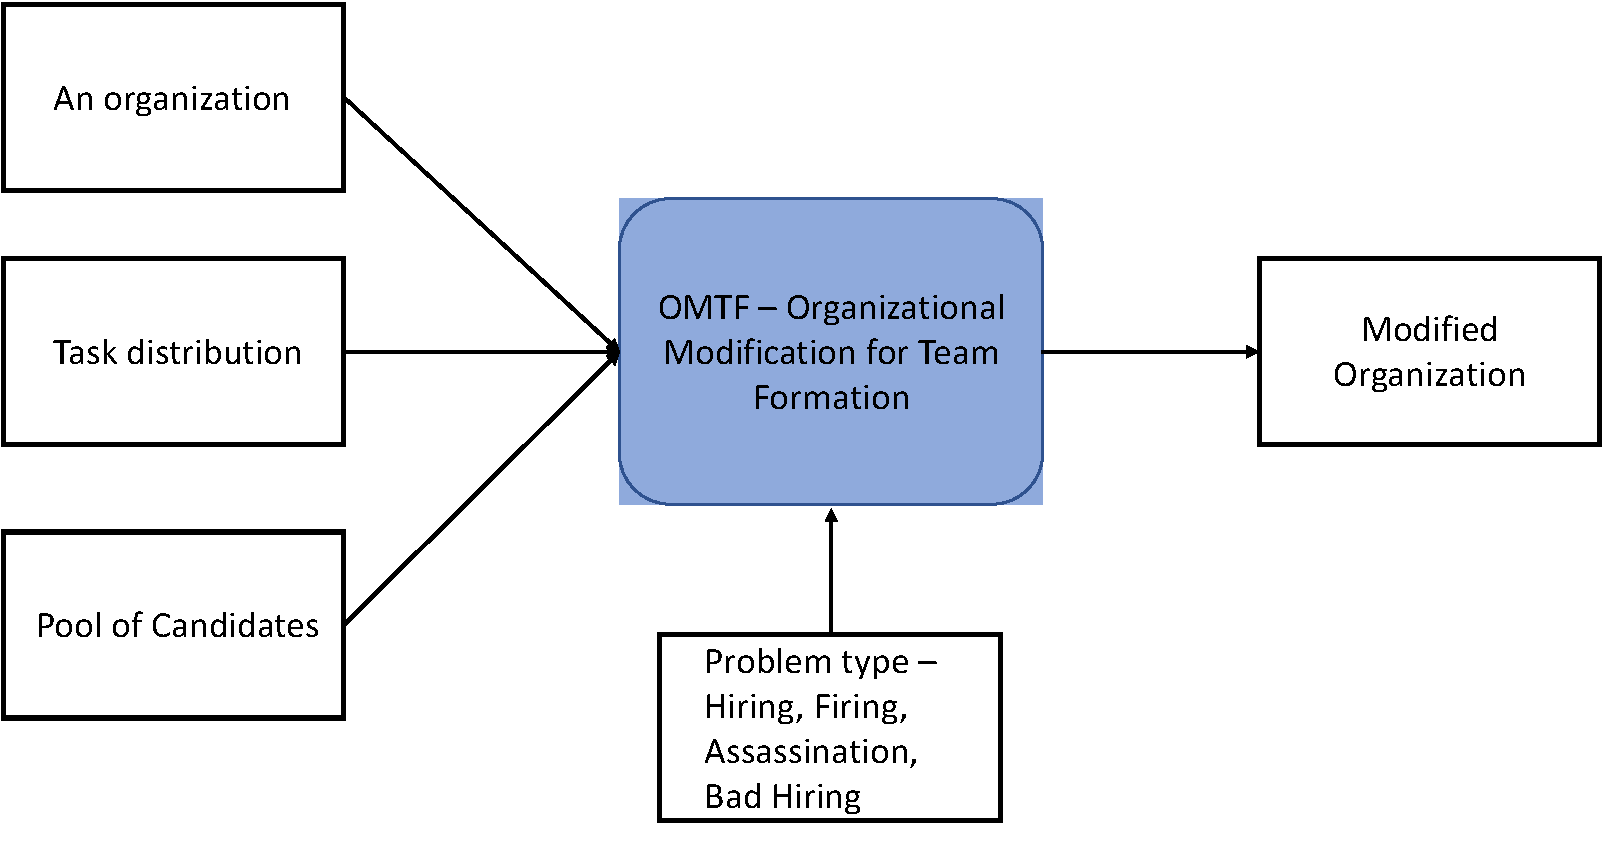
\includegraphics[width=1.0\textwidth]{figs/illustration.pdf}
\caption{Framework of our proposed system}
\label{fig:hpo}
\end{small}
\end{figure} 

Unfortunately optimizing all the four objectives are NP-hard. Hence we resort to approximation strategies. Recently in \cite{bai2016algorithms} authors have produced a simple greedy approximation that preserves a $1 - \frac{1}{e}$ - approximation while optimizing an objective that is ratio of submodular functions. Now under properly chosen utility and cost functions, the objective of team formation problem turns out to be a ratio of submodular functions. Thus we base our algorithm to that approach. However presence of organization creates an added layer of complexity. Our aim is to optimize the decision we make for the organization, which in turn depends on optimum allocation of the resources to the tasks. The second optimization can be approximated using the proposed algorithm of \cite{bai2016algorithms}. However presence of the outer optimization breaks the approximation guarantee. To circumvent this issue, we use greedy heuristics, that leverage the combinatorial structure of the problems. This algorithm does not have a provable bound, but we show that in real world datasets it performs quite well.

Thus, to summarize, our contributions are the following:

\begin{enumerate}
\item We formulate the novel \textit{hiring, firing, assassination and bad hiring problems}, in context of an organization, which draws inspirations from the team formation literature.

\item We show that the problems are NP-hard. However, under certain communication and coverage functions we can get, efficient approximation algorithms can be designed for the problems.

\item By leveraging the work of \cite{bai2016algorithms}, we develop a greedy heuristic to solve the problems. We show that because of the presence of an additional optimization requirement, the $(1 - \frac{1}{e})$ approximation guarantee of \cite{bai2016algorithms} does not carry forward. However by exploiting the combinatorial nature of our problem we develop an efficient greedy heuristic.

\item We experimentally validate our approach on real world dataset. 

\end{enumerate}
\section{Related work}
Team formation (TF) problem in the context of a social network, was first introduced by Lappas et al. in \cite{lappas2009finding}. They established that under two different communication costs, namely \textit{minimum spanning tree} (MST) and \textit{diameter} (DIA), the TF problem turns out to be NP-hard. By exploiting the connections with existing combinatorial problems such as \textit{set cover}, they developed greedy heuristics that are shown to perform well in real-world datasets. In a series of follow up works \cite{anagnostopoulos2010power,kargar2011discovering,anagnostopoulos2012online,majumder2012capacitated,kargar2012efficient,kargar2013finding}, more realistic constraints and different cost functions have been studied. In \cite{kargar2011discovering}, Kargar et al proposed a version of the problem where a team of expert is selected with a \textit{leader}, and also studied it in light of two new cost functions based on the sum of distances and leader distance. Later in \cite{kargar2012efficient,kargar2013finding} authors take into account personnel costs, and formulates the bi-objective as the linear combination of communication costs and personnel costs. 

In \cite{anagnostopoulos2010power} Anagnostopoulos et al. devised an algorithm to keep the workload balanced. In \cite{anagnostopoulos2012online} they study an online version of the problem where tasks stream and once an allocation decision is made, it cannot be revoked. Majumder et al. in \cite{majumder2012capacitated}, focuses on the TF variant where workers have a maximum capacity of tasks that they can work on simultaneously. In \cite{rangapuram2013towards} authors incorporate more ``realistic'' constraints, such as team leaders, max team sizes, and geographic locality. Their formulation results in a generalized version of the ``densest subgraph problem'' with cardinality constraints, for which they then develop an approximation via a continuous relaxation. Bhowmik et al in \cite{bhowmik2014submodularity}, generalizes previous variants of TF under a single framework. They show that it's an unconstrained submodular function maximization problem, though it is non-monotone. Their generalizations include accounting for optional skills, allowing communication to go outside the team, and relaxing the constraint that the whole team is connected. More recently in \cite{farasat2016social}, authors use TF with costs based on network structures. They rehash the Team Formation Problem from the perspective of ideas in social networks. However, none of these problems takes into account the presence of an organization. Further, the tasks are deterministic. In our problem, we solve the problem for an expected task requirement for an existing organization.

The wide variety in TF problem also sparked interest in benchmarking the algorithms and testing their effectiveness on a unified data source. In \cite{wang2015comparative} authors compare performances of different TF algorithms. They use DBLP dataset to test the algorithms. In our paper we also used the same dataset to maintain the consistency.

We formulate our problem as a maximizing ratio of submodular functions. Greedy approximation that preserves $( 1 - \frac{1}{e})$ approximation guarantee was presented in \cite{bai2016algorithms}. However, the presence of organization poses an additional complexity in the objective. Hence the same approximation guarantee does not carry forward. 

Apart from team formation another interesting problem which has similarity to ours is scheduling with load balancing. In that domain, a well-studied problem
since the work of Graham \cite{graham1972bounds}, is the scheduling of jobs on
a set of machines with the goal of minimizing the maximum
load on a machine. The setting has been extended to the
restricted-assignment problem, in which the goal of balancing
the workload is kept but additionally each job can only
be processed by a subset of the available machines. The latter
problem is NP-hard and has competitive ratio $O(ln k)$
(where $k$ is the number of jobs), shown to be asymptotically
tight even for randomized online algorithms \cite{aspnes1993line,azar1995competitiveness}. Our
work deals with a problem harder than restricted assignment. All of our objectives have
underlying theme of forming a team which in turn entails solving a set-cover problem, that has additional logarithmic lower-bound factors
even in the offline case \cite{sleator1985amortized}.

\section{Definitions and problem statement}\label{sec:pf}
In this section we formally define the notation and the problem we will be dealing with.
\subsection{Set-up}

\subsubsection{Person and skill}

We consider the input to our problem to include an existing organization.
We use the notation $\hiredset$ to denote the set of individuals who are already part of the organization.
Additionally, a set of candidates is denoted by $\candidates$.
Every individual person $p \in \{\hiredset \cup \candidates\}$ has a set of skills, a cost to be hired, and a cost to be included in a team (eg a node weight).
We use $\skill(p)$ to denote the skills of person $p$, $c_H(p)$ as the hiring cost, and $c_T(p)$ as the team cost.
The skills of a set of persons $\persons$ is $\skill(\persons) = \cup_{p \in \persons} \skill(p)$.

The universe of skills is denoted by the set $\skills = \{ s_1, ..., s_m \}$, where $s_i$ denotes $i$-th skill.

\subsubsection{Task Distribution}

A task $\task$ is nothing but the set of skills that are required to complete the task.
We write $\skill_i \in \task$ if $\skill_i$ is required to complete the task $\task$.

Most organizations cannot predict in advance the exact requirements of the tasks that will be requested.
We model this uncertainty using a task distribution $\tasks$. 
A task $\task \sim \tasks$ is associated with a probability.
Define $Pr[\task]$ to denote the probability with which the organization will be required to complete the task $\task$. 
%As the organization wishes to maximize the number of tasks it completes, it naturally places higher priority on being able to complete high probability tasks.


\subsubsection{Communication Cost}
For a subset of individuals, the communication costs can be measured in different ways. 
For a set of individuals $\persons$, we denote the communication cost as $\cost(\persons)$. 
In \cite{lappas2009finding}, the diameter of the graph and minimum spanning tree (MST) are used as two different communication costs.
Many of the subsequent team formation papers study these same two measurements.
In our paper, however, we start with a simpler cost, which is just the sum of node weights. We chose the sum of node weights as our cost function as it is modular and monotone which is more amenable to analysis with existing techniques. 

\subsubsection{Utility}
Unlike communication cost, the utility of a subset of individuals depends on the task they aim to perform. 
For a task $\task$, coverage $\cov(\persons,\task)$ is the subset of skills that a team $\persons$ possess.
More formally $\cov(\persons,\task) = |\skill(\persons) \cap \task|$.
The utility of a team $ \persons $ is $\util(\persons,\task) = \frac{\cov(\persons, \task)}{|\task|}$.

To take into account the conflicting objectives of maximizing the utility of completing the task and minimizing the communication cost of the given team, we introduce the notion of value. We define the value of a team to be the ratio of the utility over the cost and maximize this value. Notice that maximizing the ratio of two functions is equivalent to minimizing their reciprocal.  

We define the value of a task for a given organization (graph) $G$ as $TF(G,\task) = \max_{\persons \subseteq G}{val(\persons,\task)}$. We can now extend the notion of value to the expected value of a team over the task distribution. There we define $val(\persons,\task)$ to be $\frac{\util(\persons,\tasks)}{cost(\persons)} $

Thus the expected value for the organization over the task distribution is said to be as follows.

$$\mathbb{E}[TF(G,\task)] = max_{\persons \subseteq G} \left\{ \frac{\sum_{\task \sim \tasks } Pr[\task] \times \util(\persons, \task)} {\cost(\persons)} \right\} $$ \\

Note that the numerator is a non-negative linear combination of a monotone submodular function and is also submodular.

Equipped with these definitions, we are now ready to formally introduce the problems that we study in this paper.

\subsection{Problems}

In this section we present the problems we studied and the analyse the connections between them. For the ease of exposition, we define the hiring problem first i.e., given a set of candidates and a hiring budget, who do we expect to be the best candidates to hire. The other problems (i.e. firing, assassination and bad hiring) are described using the same notations. We explicitly mention the notations that are specific to certain problems.

\subsubsection{Hiring problem}

For this problem we consider as input: an existing organization of people $\hiredset$, a candidate pool $\candidates$ from which to select new hires to the organization, and a budget $B$ that denotes the maximum amount that can be spent on hiring candidates.
We use cost and utility functions as defined above to define the problem generally as follows:
\begin{problem}
[HireMax] Given $\hiredset$, communication cost $\cost$ between every pair of individuals, a distribution of tasks $\tasks$ and a budget $B$, hire a candidate set $X$ that maximizes our organizations expected value and does not exceed our hiring budget. Thus find a $X$ such that,

$$ \max \mathbb{E}[TF(G,\task)]  $$
$$ G=\hiredset  \cup X \quad c_H(X) \le B \quad X \subseteq C $$

where $c_H(X) = \sum_{x \in X} c_H(x)$ is the hiring cost of the set X.
 
\end{problem}

We now show that $HireMax$ is NP-Hard.

\begin{theorem} \label{thm:HM-hardness}
HireMax is NP-Hard.
\end{theorem}

\begin{proof}
It is easy to see that to solve this problem we must solve the underlying team formation problem. Even if the underlying team formation problem is restricted to a constant cost function, this problem requires maximizing the coverage function. This is an example of submodular maximization of a monotone function under knapsack constraint, which is known to be NP-Hard.  
\end{proof}

\subsubsection{Alternative Formulations}

From the formulation of the hiring problem three alternative problems naturally present themselves. The one which is naturally counter to hiring, is the problem of firing existing employees is presented below.  

Given an organization $\hireset$, a candidate pool $\candidates$ (often the whole organization), and a quota $Q$ we aim to fire a subset  of $\candidates$ such that we free up at least $Q$ of our budget quota and we do the least damage to the organization's value. Formally find a set $X$ that, 

$$ \min \mathbb{E}[TF(G,\task)] $$
$$ G = \hiredset \setminus X \quad Q \le c_H(X) \quad  X \subseteq C $$

The third version of the problem deals with the rivalry between two organizations. An organization could be trying to assassinate some subset of the $\candidates$, from a rival organization so that the most damage is done in terms of rivals value. Again $B$ denotes the budget that can be spent on assassination, $C$ is the candidate set that can be assassinated. Then the objective is to find a set $X$, such that

$$ \max \mathbb{E}[TF(G,\task)] $$
$$ G = \hiredset \setminus X \quad c_H(X) \le B \quad  X \subseteq C $$

Our last problem follows by the symmetry, but does not have a strong motivation, is hiring a set of candidates that adds minimum value to the organization. Here a budget quota $Q$ is given that denotes the number of bad hires that has to be made from a candidate set $C$. Thus formally the goal is to find a set $X$ such that,

$$ \min \mathbb{E}[TF(G,\task)] $$
$$ G = \hiredset \cup X \quad Q \le c_H(X) \quad  X \subseteq C $$

\subsubsection{A remark on the hardness of the alternative formulations}

Note that in all three versions we still need to solve the central team formation problem optimally. Thus the core argument of  the proof of theorem \ref{thm:HM-hardness} carries forward - under constant cost we need to maximize the coverage function, which is NP-hard. Hence all these three problems are NP-hard.

\bibliographystyle{abbrv}
\bibliography{bib/paper}  % sigproc.bib is the name of the Bibliography in this case

\end{document}





